% This must be in the first 5 lines to tell arXiv to use pdfLaTeX, which is strongly recommended.
\pdfoutput=1
\documentclass[11pt]{article}
\usepackage{ACL2023}
\usepackage{times}
\usepackage{latexsym}

% For proper rendering and hyphenation of words containing Latin characters (including in bib files)https://www.overleaf.com/project/65552408b47f56013140e936
\usepackage[T1]{fontenc}

% This assumes your files are encoded as UTF8
\usepackage[utf8]{inputenc}

% This is not strictly necessary, and may be commented out.
% However, it will improve the layout of the manuscript,
% and will typically save some space.
\usepackage{microtype}

% This is also not strictly necessary, and may be commented out.
% However, it will improve the aesthetics of text in
% the typewriter font.
\usepackage{inconsolata}

% graphics package
\usepackage{graphicx}
\usepackage{placeins}  % table across columns
\pagestyle{plain}
\usepackage{float}
\usepackage{multicol}
\newcommand{\justifylastline}{\setlength{\parfillskip}{0pt}}

% If the title and author information does not fit in the area allocated, uncomment the following
%
%\setlength\titlebox{<dim>}
%
% and set <dim> to something 5cm or larger.

% More packages
\usepackage{graphicx} % Required for including images
\usepackage{caption}  % Required for \captionof
\usepackage{booktabs} % For prettier tables
\usepackage{amsmath}  % For math symbols and equations
\usepackage{geometry} % For page dimensions and margins

\title{Biomedical Literature Review Summaries Using Multi-Document Summarization}
\author{
  \begin{tabular}{c}
    Farid Gholitabar \\
    {\small\texttt{farid.gholitabar@berkeley.edu}}
  \end{tabular}\and
  \begin{tabular}{c}
    Mike Khor \\
    {\small\texttt{mike.khor@berkeley.edu}}
  \end{tabular}\and
  \begin{tabular}{c}
    Amir Moazami \\
    {\small\texttt{amirmoazami@berkeley.edu}}
  \end{tabular}\\\\
  University of California Berkeley
}

\date{December 2023}

\begin{document}
\bibliographystyle{unsrt}

\maketitle
\begin{abstract}
This research leverages multi-document summarization (MDS) to enhance literature review methods in the biomedical domain, aiming to generate concise, informative abstracts from diverse biomedical literature. We address challenges such as reconciling conflicting findings, managing complex terminology, and handling large datasets. Our approach integrates new and advanced NLP analysis techniques for deeper understanding than traditional methods. A hybrid extractive-abstractive model, incorporating innovative techniques tailored to biomedical literature, effectively condenses information into comprehensive summaries. Our findings highlight the high performance of the PEFT BioBERT + K-means + LongT5 model for short target sentences, suggesting promising avenues for future research. This work represents a significant step towards more efficient literature review methodologies and showcases the transformative potential of MDS in biomedical research.
\end{abstract}

\section{Introduction}

The exponential growth of biomedical research literature presents a formidable challenge for researchers to stay abreast of the latest developments and findings. Conducting literature reviews is a fundamental component in the biomedical domain and essential for assessing the efficacy and safety of medical interventions. However, this process is highly time-consuming, often taking approximately one to two years to review and synthesize information from individual medical studies thoroughly. The necessity for efficient and accurate methods to expedite this process is more pressing than ever.

Our project aims to address this challenge by applying multi-document summarization (MDS) techniques. Specifically, we propose to use MDS to create concise, coherent abstracts of literature reviews for biomedical journal topics. We aim to streamline the summarization of multiple related medical studies and their subsequent updates by employing existing algorithms and datasets.

Key challenges include: \textbf{i) conflicting findings}: varying and sometimes conflicting results in biomedical studies; \textbf{ii) complex vocabulary}: specialized lexicon of the biomedical field necessitating a deep understanding; \textbf{iii) long sequences}: handling a variable number of input studies, sometimes exceeding 20, requires robust data engineering and processing strategies.

Our research aims to understand and tackle these challenges and provide an MDS solution that enhances literature review processes. We hope to aid medical professionals and researchers in making informed decisions based on a short yet comprehensive summary of existing medical literature.


\section{Background}

\subsection{Related Work and Previous Research}

Popular summarization datasets (i.e., Multi-XScience \cite{lu2020multixscience}) are not specific to biomedical texts, whereas the “Cochrane” biomedical summarization dataset \cite{wallace2020generating} lacks in size. Recently, the “Multi-Document Summarization of Medical Studies,” MSˆ2 dataset \cite{deyoung2021ms2} emerged, containing over 470,000 documents and 20,000 summaries. This large-scale public dataset facilitates automated biomedical MDS development and has sparked research efforts (\cite{otmakhova2022m3, tangsali2022abstractive, shinde-etal-2022-extractive}).

MDS techniques are diverse, encompassing a range of methods from graph-based approaches that leverage textual connections to context-based strategies that integrate broader meanings. For an insightful overview of these techniques, Ma et al. (\cite{ma2020multidocsum}) provide comprehensive coverage. Foundational models like Bi-directional and Auto-Regressive Transformers (BART) have been instrumental in advancing abstractive summarization methods. However, the exploration of hybrid multistage extractive-abstractive approaches, which combine the strengths of both extractive and abstractive methods, has been relatively limited. Such hybrid methods typically utilize an extractive step to condense input lengths, followed by an abstractive model to generate the final summary output. A notable example of this technique is WikiSum (\cite{liu2018generating}), which employs an initial extractive process to identify key information and then generates a summary based on these highlights. To date, Shinde et al. (\cite{shinde-etal-2022-extractive}) are among the few who have investigated the application of multistage summarization in biomedical literature, specifically using the Cochrane dataset. Their approach combines a BERT-based extractive method with PEGASUS for abstractive summarization.


\begin{figure}[h]
  \centering
  \includegraphics[width=\linewidth]{fig1.jpg}
  \caption{Given study abstracts and a BACKGROUND statement, generate the TARGET summary. Diagram from \cite{deyoung2021ms2}.}
  \label{fig:ms2-explainer}
\end{figure}
\vspace{-15pt} % Adjust the value as needed

\subsection{How is Our Work Different?}

In our research, we introduce extractive-abstractive summarization tailored for the MSˆ2 dataset and offer a detailed comparative analysis of the choices of the extractive and abstractive components. By selectively parsing critical data from diverse abstracts using extractive summarization, our method overcomes the input length limitations of pure abstractive models. This refined approach enhances the quality of abstractive model output summaries.

In addition, we present several finetuning efforts on the chosen abstractive model. We highlight some important considerations for finetuning and detail the limitations of finetuned summaries.


\section{Methods}

\subsection{Data Acquisition and Preprocessing}

MSˆ2 contains 20K biomedical literature reviews (examples), and each review contains a background on the topic of interest, a list of studies referenced in the review, the studies’ abstracts, and a target summary (text extracted from the “abstract” portion of the review) (Figure~\ref{fig:ms2-explainer}). We used the dataset’s pre-split of training and validation sets but excluded the test pre-split because it lacks targets (used for leaderboard benchmarking). Prior to extractive summarization, MSˆ2 studies’ abstracts are separated into sentences using the Scispacy module, a model trained explicitly on scientific literature.


\subsection{Baseline Models}
We employed extractive and abstractive models separately before progressing to a hybrid model to assess the individual strengths of each model type in isolation.

We assessed BERT\cite{devlin2019bert}, BioBERT\cite{Lee_2019}, and SciBERT\cite{beltagy2019scibert} models for extractive summarization, which provide a semantic understanding of individual sentences. We used K-means to cluster sentence-level BERT embeddings per study to pinpoint the most pertinent sentences and phrases. Then, we picked one representative sentence from each cluster, as inspired by \cite{miller2019leveraging}. This extractive technique retrieves sentences of diverse semantic meanings while leaving out redundant sentences. The choice of BERT encoders depends on their ability to understand complex biomedical topics and catch nuanced details.

We selected Pegasus\cite{zhang2020pegasus}, BioBART\cite{yuan2022biobart}, and LongT5\cite{guo2022longt5} models for abstractive summarization, which are proficient in generating coherent abstractive summaries. These models have constraints, such as Pegasus and BioBART's restricted input token length, which can hinder their ability to process longer documents. BioBART, while tailored for biomedical texts, could struggle with highly specialized or rare medical terminology not covered in its training dataset.

Please see Appendix~\ref{app:baselineoverview} for a more detailed description of the abovementioned models.

\subsection{Evaluation Methods}

Our study utilized a specific segment of our dataset to evaluate model effectiveness in summarization tasks. The metrics employed were \textbf{ROUGE}, \textbf{BERTScore}, and \textbf{\(\Delta\)EI} (Evidence Inference Delta). Specifically, \(\Delta\)EI, as delineated in MSˆ2 \cite{deyoung2021ms2}, utilizes a Biomed-RoBERTa-based model to calculate probabilities across three evidence directions: "significantly decreases," "no significant difference," or "significantly increases." This metric evaluates the divergence in these probabilities between the target text and our generated summaries. A lower \(\Delta\)EI score signifies greater agreement in the direction of evidence, reflecting the accuracy of our summarization models in capturing evidence directions.


\subsection{Experimental Methods}

Our research explored two distinct experimental methods, each employing a hybrid of extractive and abstractive techniques but with different approaches to either component. Each outlined experiment’s architecture overview can be found in Appendix~\ref{app:schematics}.

\subsubsection{Experiment 1: Hybrid Extractive-Abstractive Technique Using BioBERT and K-means Clustering with LongT5}
\label{exp:1}
Leveraging the synergy between BioBERT's advanced capabilities and K-means clustering for processing biomedical literature, our research employed a hybrid extractive-abstractive technique. This extracted text segment was then subjected to the Long T5 model.

We utilized K-means clustering to identify and select the most informative sentences in each abstract. We could isolate key sentences in each abstract by fitting the sentence embeddings into a K-means model configured with a specific number of clusters to match our desired sentence count. A unique aspect of our approach was ensuring that each chosen sentence came from a different cluster, thereby enhancing the diversity and relevance of our extracted content.

In the next phase, we concatenated the selected sentences to form extractive summaries and then fed them into LongT5, resulting in succinct abstractive summaries.

\subsubsection{Experiment 2: Text Clustering and Summarization using BioBERT, UMAP, HDBSCAN, and LongT5}
First, we used BioBERT to generate sentence embeddings, consistent with our previous approach. Next, we explore a different clustering technique for extracting key sentences, using Hierarchical Density-based Spatial Clustering of Applications with Noise (HDBSCAN)\cite{asyaky2021hdbscan}, which handles noise well and efficiently manages different data densities.

However, HDBSCAN struggles with high-dimensional data. To overcome this, we incorporated Uniform Manifold Approximation and Projection (UMAP) for dimension reduction, which retains density information, a critical aspect often lost in other dimension reduction methods.

Like K-Means extraction, one key sentence is extracted from each cluster of sentences and concatenated before being fed into LongT5.

\subsubsection{Experiment 3: Rule-based Extractive Summarization Using Targeted Keyword Search}
As a more straightforward extractive approach, our "extractive model" in this experiment was designed to search specifically for the word "conclusion" within the texts for each abstract. Upon locating this term, the model extracted the sentence containing it and any subsequent sentences in the abstract. This approach was based on the hypothesis that sentences following the term "conclusion" in scientific literature are likely to contain key summary points of the research.

After extracting these segments, we feed them into LongT5 to synthesize a cohesive summary. This method leverages the inherent structure of scientific abstracts and mimics how a human reviewer would approach this summarization problem.

\subsubsection{Experiment 4: Extractive-Abstractive Summarization with BioBERT, K-means Clustering, and Fine-Tuned LongT5}
In this experiment, we employed a two-phase training process for the LongT5 model, with each phase addressing different data representations.

During the initial phase, we trained the LongT5 model on the raw training data from the MSˆ2 dataset. This training, executed over 8 epochs, was strategically focused on minimizing cross-entropy loss. A notable constraint encountered was the model's limited input capacity, compounded by our computational resource limitations. Consequently, we were restricted to input data comprising 2,048 tokens for each training instance. However, this experiment led us to explore an alternative training approach in the second phase.

The second phase involved training the LongT5 model on a transformed version of the training data. We first processed the data through BioBERT for embedding, followed by the K-means, which provided a compressed and more focused representation of the input data. (how it was explained earlier in other experiments) This approach aimed to encapsulate the essential information effectively within the model’s input capacity limits. We hypothesized that this representation would enable more comprehensive learning from the dataset. This phase of training also spanned 7 epochs.

To rigorously evaluate the model's performance in each phase, we utilized two distinct sets of validation data. The first set entailed assessing the summarization capabilities of each model iteration using the unprocessed validation dataset. In contrast, the second set involved validation data that had undergone preprocessing through BioBERT embedding, followed by K-means clustering. This approach, aimed at creating a condensed and refined version of the input data, is indicative of a potential operational data pipeline for the model’s inferences. Our dual-method testing approach was instrumental in thoroughly evaluating the model’s proficiency in processing and summarizing both raw and pre-processed biomedical texts.

\subsubsection{Experiment 5: Extractive-Abstractive Summarization with BioBERT, K-means Clustering, and PEFT LongT5}

Lastly, we used a Parameter Efficient Fine-Tuning (PEFT) method, Low-Rank Adaptation (LoRA) to finetune \textit{BioBERT-K-means-LongT5}. LoRA significantly reduces the number of parameters needed to fine-tune a pretrained model, drastically reducing memory usage during training \cite{hu2021lora}. The motivation for using LoRA stems from memory constraints encountered in full fine-tuning (the last experiment), in which the input tokens had to be truncated down from 16,384 to 2,048. With LoRA, we were able to fine-tune LongT5 with a longer input length of 8,192 using the same hardware. This longer input length means that only 5.3\% of our BioBERT-K-means extractive summaries were truncated prior to LongT5 abstractive summarization.


PEFT LoRA was applied to all query and key weights for all 11 transformer layers (both encoder and decoder). Keeping our LongT5’s original 247 million parameters frozen, we added an additional 1.7 million LoRA parameters, which means only 0.7\% of parameters are trainable. The PEFT model is then trained on the training dataset for 4 epochs.

\section{Results and Discussion}

\subsection{Choosing Appropriate Abstractive and Extractive Models}
For abstractive summarization, this research evaluated Pegasus, BioBART, and LongT5 (Table~\ref{tab:baseline_model_evaluation}). LongT5 is chosen due to its higher BERTscore average F1 and ROUGE-1 F1 scores, which indicate better performance in generating coherent, context-rich summaries. A significant advantage of LongT5 is its ability to process longer texts, which is crucial for handling extensive biomedical literature without needing data engineering modifications like restricting attention mechanisms. Its mixed attention mechanism, blending local and sparse global attention, is noted for efficiently handling large datasets, making it suitable for extensive text summarization tasks.

For extractive summarization, we selected BioBERT combined with K-means clustering for its low $\Delta$EI average score of .503. This score reflects BioBERT's superior factual accuracy and alignment with target summaries. BioBERT's training in biomedical literature is a key factor in its performance, as it enables a nuanced understanding of biomedical contexts. This aspect is particularly valuable for information extraction from complex biomedical texts.


\subsection{Evaluating the Combination of Extractive and Abstractive Models}
We assessed three unique combinations of integrating extractive and abstractive methods: 1) \textit{Rule-based + LongT5}, 2) \textit{BioBERT + K-means + LongT5}, and 3) \textit{BioBERT + UMAP + HDBSCAN + LongT5}. Notably, these combined models outperformed standalone BioBERT-K-means or LongT5, highlighting the complementary strengths of both approaches. The K-means algorithm effectively reduced input lengths for LongT5, improving attention management. LongT5 then condenses content into more precise outputs, thereby improving ROUGE precision.

ROUGE score analysis highlighted that the \textit{BioBERT + UMAP + HDBSCAN + LongT5} model underperformed, often paraphrasing content and omitting key phrases or terms. In contrast, BERTScore evaluation, which focuses on semantic similarity, identified \textit{Rule-based + LongT5} as more effective at capturing the essential semantic content despite lower ROUGE scores.

\justifylastline
The $\Delta$EI scores pointed to moderate inconsistencies in factual accuracy across all models compared to the pure extractive method. Of the three combinations, \textit{BioBERT + K-means + LongT5} scored the lowest (best) $\Delta$EI (.519) and preserved factual details better than the pure abstractive method ($\Delta$EI = .543), as a contribution of BioBERT-K-Means. The model's effectiveness likely stems from the synergistic combination of BioBERT's understanding of biomedical contexts, K-means clustering efficiency, and LongT5 summarization. This blend facilitates
\FloatBarrier
\begin{table*}[h!]
  \centering
  \small
  \begin{tabular}{clcccccc}
    \toprule
    Experiment & Model & R-1  & R-2 & R-L & BERT & $\Delta$EI & $\Delta$EI \\
    & & & & & score & average & macro F1 \\
    \midrule
    Baseline & LongT5 & .185 & .022 & .106 & .543 & .543& .364 \\
    Baseline & BioBERT + K means & .046 & .012 & .029 & .502 & .503 & \textbf{.389}\\
    1 & BioBERT + K means - LongT5 & .194 & .024 & .109 & .550 & .519 & .382 \\
    2 & BioBERT + UMAP + HDBSCAN + LongT5 & .187 & .023 & .105 & .545& .559 & .363 \\
    3 & Rule-based (conclusion-focused) + LongT5 & \textbf{.210} & \textbf{.028} & \textbf{.125} & .567 & .526 & .377\\
    4 & Full Fine-Tuned LongT5 & .154 & .022 & .115 & .561 & .576 & .332 \\
    4 & BioBERT + K means - Full Fine-Tuned LongT5 & .148 & .018 & .110 & .558 & .568 & .331 \\
    5 & BioBERT + K means - PEFT Tuned LongT5 & .181 & \textbf{.028}& .134 & \textbf{.591} & \textbf{.453}& .362 \\
    \bottomrule
  \end{tabular}
  \caption{Model evaluation results. BERTscore values are average F1. Values in bold indicate the best model.}
  \label{tab:model_evaluation_all}
\end{table*}
\FloatBarrier
\setlength{\parfillskip}{0pt plus 1fil}

\noindent a ‘deep’ semantic understanding of sentence meanings during clustering, and a ‘broad’ ability to handle extended inputs with LongT5’s localized-global sparse attention.

We hypothesize that the suboptimal performance of \textit{BioBERT + UMAP + HDBSCAN + LongT5} is due to UMAP dimensionality reduction, which might lead to the loss of critical keywords or phrases, as suggested by its lower ROUGE scores.

\subsection{Improving the extractive-abstractive combination model via fine-tuning}
\subsubsection{Full Fine-Tuning (FFT)}
After selecting \textit{BioBERT + K-means + LongT5} as the most performant architecture, we performed full fine-tuning, FFT (Experiment 4). In all FFT cases, we observe a decrease in performance in ROUGE-1, ROUGE-2, $\Delta$EI average, and EI macro F1 (Table~\ref{tab:model_evaluation_all}). FFT models struggle to predict the direction of the medical outcome (EI) and cannot produce relevant tokens after abstraction (ROUGE-1, ROUGE-2). FFT’s BERTscore and ROUGE-L have insignificant changes.

One hypothesis for the degradation of performance lies in the hardware-constrained input length limit. By truncating input lengths from 16,384 to 2,048 tokens during training, 71\% of training examples after extractive summarization are shortened to the first 2,048 tokens for abstractive summarization (see Figure~\ref{fig:kmeans_summary_lengths} in Appendix~\ref{app:relevantdata} for a visualization of the extent of truncation). If a literature review has many referenced studies, this truncation could lead to a training input-output pair where the input does not contain the signal needed to inform its output, effectively causing data quality issues. Appendix~\ref{app:relevantdata} Table~\ref{tab:fft_worst_bert} shows an example where an FFT-generated summary only contains information from the first study.

Additionally, in the context of FFT with truncated inputs, K-means extractive summarization has a neutral or mildly negative effect on model performance, regardless of whether it is used during training/fine-tuning, inference, or both (Appendix~\ref{app:relevantdata}, Table~\ref{tab:fft_comparison}), which contradicts our non-FFT model learnings (adding K-means extractive summarization improves LongT5). One possible explanation is that FFT models can exhibit extractive capabilities by adjusting their attention weights to focus on crucial tokens or phrases needed for medical summaries, negating the need for K-means extractive summarization.

\subsubsection{Parameter-Efficient Fine Tuning (PEFT)}

In \textit{BioBERT + K-means + PEFT LongT5} (Experiment 5), we see a marked improvement in BERTscore, $\Delta$EI, and ROUGE-L compared to its non-finetuned counterpart (Table~\ref{tab:model_evaluation_all}). These improvements highlight the importance of having a large input length and PEFT’s role in enabling it.

However, the PEFT model underperformed relative to the non-finetuned variant in EI macro-averaged F1, despite an observed decrease (improvement) in the $\Delta$EI average. $\Delta$EI, a classification-based evaluation, classifies each target and generated summary into three evidence directions. Analysis of the classification report for summaries generated by the PEFT model (Appendix~\ref{app:relevantdata}, Table~\ref{tab:peft_classification_report}) revealed a notable class imbalance, dominated by targets classified as “no significant difference.” This imbalance in the training dataset led to improved scores for the majority class (“no significant difference”) but also deteriorated scores for the other two classes, leading to a lower macro F1. The PEFT model takes shortcuts to cross-entropy loss by over-generating summaries that imply insignificant medical outcomes. Future work should address this class imbalance using traditional class-balancing techniques (down-sampling, class-balanced loss).

Oddly, after FFT or PEFT/LoRA, generated summaries are shorter than those generated by its non-finetuned version (Experiment 1) or target summaries (Figure~\ref{fig:summary_lengths_comparison}). The distribution of finetuned summary lengths centers around the targets’ mode length, which means that the finetuned models learned the most common positional information for generating a stop token. Our finetuned models cannot generate more extended summaries (e.g., medical reviews that investigate multiple outcomes). Unsurprisingly, this effect increases precision but decreases recall for ROUGE scores and BERTscore (Appendix~\ref{app:relevantdata}, Figure~\ref{fig:peft_score_shifts}).

At a high level, an example-level difference in metric scores between pairs of models is available in Appendix~\ref{app:pairwise-model-comparison}.

\section{Discussion}
\subsection{Balancing Factual Accuracy with Semantic Coherence}

Our study highlights the complex relationship between factual accuracy and semantic coherence in biomedical summarization. The impressive performance of the \textit{PEFT BioBERT + K-means + LongT5} model demonstrates the benefits of a comprehensive approach that melds context understanding, efficient data clustering, and advanced summarization techniques. Notably, the model's memory efficiency plays a critical role in processing larger data sets, significantly enhancing the quality of our summaries. This underlines the importance of accommodating substantial input lengths in MDS tasks. The findings emphasize the crucial influence of computational efficiency in improving the outputs of such models.

\subsection{Comparative Analysis of Extractive and Abstractive Models}

The BioBERT + K-means model maintained factual accuracy, as evidenced by its superior $\Delta$EI score. In contrast, the LongT5 model demonstrated prowess in generating contextually rich summaries. The mixed attention mechanism of LongT5 was crucial in efficiently processing larger datasets.

\subsection{Dealing with Diverse Summaries in the MSˆ2 Dataset}

The MSˆ2 dataset, notable for its varied summary targets, poses significant challenges. Analysis (Appendix~\ref{app:relevantdata} Table~\ref{tab:best-worst-peft}) shows that the PEFT \textit{BioBERT + K-means + LongT5} model excels with shorter summaries, as indicated by high BERTscores, but struggles with longer ones. The dataset's target sentences, derived from review article abstracts using a SciBERT-based model and human annotations, sometimes inadvertently include complex parts from the results section, leading to target length irregularity. Improving the consistency of target generation could improve data quality and increase the relevance of our summarization efforts.

\begin{figure}[h!]
    \centering
    \includegraphics[width=1.0\linewidth]{summary_lengths.png}
    \caption{Comparison of test dataset summary length (tokens) between targets and variations of \textit{BioBERT K-means + LongT5}: no fine-tuning, FFT with K-means input, and PEFT.}
    \label{fig:summary_lengths_comparison}
\end{figure}
\vspace{-15pt} % Adjust the value as needed


\subsection{Implications and Future Directions}

We propose exploring \textbf{Retrieval-Augmented Generation (RAG) methodologies} that leverage background information (provided in MSˆ2) as a query basis to extract targeted information in studies’ abstracts (key and value). It is unclear if this method could rival BioBERT-K-means extraction.

Drawing inspiration from BioBART, a \textbf{specialized LongT5 architecture fine-tuned for biomedical terminology,} could help retain biomedical words through abstraction decoding. A “Bio-LongT5” would integrate the extensive text processing capabilities of LongT5 with a deep semantic understanding of the biomedical lexicon. Additionally, a \textbf{pointer generator} method could address the vocabulary limitations of specialized biomedical terms.

Lastly, incorporating \textbf{custom mixed loss functions with $\Delta$EI} into the training pipeline can minimize divergence in evidence directions alongside traditional cross-entropy loss. Researchers might use LongT5's encoder hidden states for classification, offering a less resource-intensive alternative to $\Delta$EI’s RoBERTa.

\section{Conclusion}
In summary, our project has made strides in the application of multi-document summarization (MDS) techniques in the biomedical domain, targeting conciseness, semantic similarity, and medical evidence directions. Our research focused on hybrid extractive (BioBERT and K-means clustering) and abstractive (LongT5) methods. We also fine-tuned our hybrid model using full fine-tuning and parameter-efficient fine-tuning (PEFT) and highlighted some challenges with fine-tuning.

The comparative analysis of our models, particularly the PEFT BioBERT + K-means + LongT5 model, has shown impressive results in balancing factual accuracy with semantic coherence. The success of this model emphasizes the critical role of large enough input lengths during fine-tuning, and the importance of memory efficiency through PEFT to enable it.

% Bibliography
\bibliography{references}
% \newpage
% \pagebreak % Insert a page break
% \bigskip
% \hrule
\section*{Appendix}
\appendix{}

\section{Overview of Baseline Models}
\label{app:baselineoverview}

\subsection*{\textbf{Pegasus} (Pre-training with Extracted Gap-sentences for Abstractive Summarization Sequence-to-sequence)}
Developed by Google, Pegasus is a model tailored for summarization tasks. It utilizes a novel pre-training strategy, where it constructs 'gap sentences' and learns to generate these absent segments. This approach specifically enhances its proficiency in producing coherent and extensive summaries. Such a feature is particularly advantageous for summarizing complex and lengthy texts, as exemplified in the MS2 dataset.

\subsection*{\textbf{BioBART} (Biomedical Bidirectional and Auto-Regressive Transformers)}
An adaptation of the BART architecture for biomedical applications, BioBART incorporates both bidirectional and autoregressive transformers. This configuration facilitates a profound comprehension of intricate biomedical contexts. Trained extensively on biomedical literature, BioBART shows a marked aptitude for summarizing complex medical texts, aligning well with the preprocessing steps designed for the MS2 dataset, particularly in processing nuanced information within the dataset's abstracts.

\subsection*{\textbf{T5} (Text-to-Text Transfer Transformer)}
T5 is predicated on the concept that all text-based tasks are convertible into a text-to-text format. This model's versatility, coupled with its comprehensive training across various language tasks, renders it an effective tool for summarization. In biomedical summarization, T5's adaptability and linguistic sophistication are essential for generating accurate and comprehensive summaries from the MS2 dataset's diverse and complex texts.

\subsection*{\textbf{BERT} (Bidirectional Encoder Representations from Transformers)}
A pioneering model in NLP, BERT was developed by Google and introduces a bidirectional training approach. Distinct from traditional unidirectional models, BERT processes text in both directions (left-to-right and right-to-left), allowing for a nuanced understanding of context and inter-sentence relationships. This characteristic makes BERT particularly effective in extractive summarization tasks, such as identifying and extracting key information from the extensive biomedical literature in the MS2 dataset.

\subsection*{\textbf{BioBERT} (Biomedical Bidirectional Encoder Representations from Transformers)}
An extension of BERT, BioBERT is pre-trained on general language corpora and extensive biomedical literature. This specialized training equips BioBERT with a heightened ability to process biomedical terminology and concepts accurately. It excels in identifying and extracting vital biomedical information, making it highly suitable for summarizing scientific articles and studies within the MS2 dataset. Its domain-specific focus enhances accuracy in handling the complex details and technical language prevalent in biomedical texts.

\subsection*{\textbf{SciBERT} (Scientific Bidirectional Encoder Representations from Transformers)}
SciBERT adapts the BERT model for the scientific domain. Pre-trained on a vast corpus of scientific literature, including papers and journals across various scientific fields, SciBERT acquires a deep understanding of scientific terminology and concepts. This pre-training makes it particularly adept at extractive summarization within scientific literature, enabling it to discern and extract relevant information from complex scientific texts, a capability that is crucial for summarizing the detailed and nuanced content in the MS2 dataset.

\bigskip
\section{Schematics of Baseline and Experimented Models}
\label{app:schematics}

\begin{center}
  \includegraphics[width=\linewidth]{1.png}
  \captionof{figure}{This diagram illustrates the use of BERT or similar models for encoding input text, followed by a K-means clustering algorithm to identify the most representative sentences, which are then used to create an extractive summary.}
  \label{fig:1}
\end{center}

\begin{center}
  \includegraphics[width=\linewidth]{2.png}
  \captionof{figure}{This diagram shows the flow of input text being processed directly by abstractive summarization models like PEGASUS, BioBART, or Long T5 to generate a literature review.}
  \label{fig:2}
\end{center}

\begin{center}
  \includegraphics[width=\linewidth]{3.png}
  \captionof{figure}{The third diagram represents a hybrid approach that uses BioBERT for text encoding and K-means for clustering to generate an extractive summary, which is then fed into the Long T5 model to create a literature review.}
  \label{fig:3}
\end{center}

\begin{center}
  \includegraphics[width=\linewidth]{4.png}
  \captionof{figure}{This diagram depicts a similar hybrid approach as Experiment 1, but with an added step of dimensionality reduction using UMAP before clustering with HDBSCAN, leading to an extractive summary that is processed by the Long T5 model.}
  \label{fig:4}
\end{center}

\begin{center}
  \includegraphics[width=\linewidth]{5.png}
  \captionof{figure}{The fifth diagram presents another hybrid approach where rule-based sentence extraction is combined with an abstractive summarization using the Long T5 model to produce a literature review.}
  \label{fig:5}
\end{center}

\begin{center}
  \includegraphics[width=\linewidth]{6.png}
  \captionof{figure}{Here, the input text is summarized abstractively using a fine-tuned Long T5 model to produce a literature review.}
  \label{fig:6}
\end{center}

\begin{center}
  \includegraphics[width=\linewidth]{7.png}
  \captionof{figure}{This diagram shows an extractive preprocessing step using BioBERT and K-means clustering to extract sentences for fine-tuning the Long T5 model, which then creates a literature review.}
  \label{fig:7}
\end{center}

\begin{center}
  \includegraphics[width=\linewidth]{8.png}
  \captionof{figure}{The final diagram describes using a BioBERT encoder with K-means clustering to perform extractive summarization. The extracted sentences are then used for fine-tuning an abstractive summarization model (PEFT Long T5) using the LORA method.}
  \label{fig:8}
\end{center}

\onecolumn

\section{Relevant Data}
\label{app:relevantdata}

\begin{figure}[h]
    \centering
    \includegraphics[width=1\linewidth]{kmeans_summary_lengths.png}
    \caption{Histogram of lengths of BioBERT K-means extractive summaries. Vertical lines indicate input limits to abstractive summarization (2,048 for full fine-tuning, 8,192 for PEFT LoRA).}
    \label{fig:kmeans_summary_lengths}
\end{figure}


\begin{table*}[h!]
  \centering
  \small
  \begin{tabular}{lcccccc}
    \toprule
    Model & R-1  & R-2 & R-L & B & $\Delta$EI & F1\\
    \midrule
    Pegasus (abs) & .174 & .019 & .109 & .522 & .558 & .360 \\
    BioBART (abs) & .158 & .036 & .093 & .525 & .526 & .378 \\
    LongT5 (abs) & .185 & .022 & .106 & .543 & .543 & .364 \\
    BERT + K means (ext) & .047 & .012 & .030 & .505 & .518 & .372 \\
    SciBERT + K means (ext) & .047 & .012 & .030 & .504 & .516 & .376 \\
    BioBERT + K means (ext) & .046 & .012 & .029 & .502 & .503 & .389 \\
    \bottomrule
  \end{tabular}
  \caption{baseline extractive and abstract Note: B = BERTscore average F1}
  \label{tab:baseline_model_evaluation}
\end{table*}

\begin{table}[h]
    \centering
    \small
    \begin{tabular}{cccccccccclll}
        \toprule
         & \multicolumn{2}{c}{R-1}&  \multicolumn{2}{c}{R-2}&  \multicolumn{2}{c}{R-L}& \multicolumn{2}{c}{BS F1}& \multicolumn{2}{c}{\(\Delta\)EI}& \multicolumn{2}{c}{EI F1}\\
         & F&K& F& K& F& K& F& K& F&K&F&K\\
         \midrule
         F&  .154&  .148&  .022&  .018&  .115&  .110&  .561&  .558&  .576& .568& .332&.331\\
         K&  .139&  .142&  .018&  .017&  .106&  .107&  .560&  .558&  .594& .580& .321&.331\\
         \bottomrule
    \end{tabular}
\caption{Metrics comparison of 4 combinations of full fine-tuned (FFT) models, where either the full dataset (F) or a K-means extracted dataset (K) is used during training (rows) and inference (columns).}
\label{tab:fft_comparison}
\end{table}

\FloatBarrier
\begin{table}[h!]
    \centering
    \small
    \begin{tabular}{cccccccc}
        \toprule
        & \multicolumn{3}{c}{BioBERT + K means + LongT5}& \multicolumn{3}{c}{BioBERT + K means + PEFT LongT5}& \\
        \midrule
        & P & R & F1 & P & R & F1 & Support\\
        significantly decreased & .117 & .194 & .146 & .103 & .072 & .085 & 111\\
        no significant difference & .636 & .548 & .589 & .626 & .778 & .694 & 1214\\
        significantly increased & .386 & .438 & .41 & .401 & .25 & .308 & 696\\
        &  &  &  &  &  &  & \\
        Accuracy &  &  & .491 &  &  & .558 & 2021\\
        Macro Average & .380 & .393 & .382 & .377 & .367 & .362 & 2021\\
        Weighted Average & .521 & .491 & .503 & .520 & .558 & .528 & 2021\\
        \bottomrule
    \end{tabular}
    \caption{Classification report of Evidence Inference for BioBERT K-means + LongT5, with and without PEFT (Experiments 1 and 5), based on test dataset.}
    \label{tab:peft_classification_report}
\end{table}

\FloatBarrier

\begin{figure}
    \centering
    \includegraphics[width=1\linewidth]{peft_score_shifts.png}
    \caption{Histograms of BERTscore, ROUGE-1, ROUGE-2, ROUGE-L, in F1, precision and recall, for two models: Experiment 1 BioBERT K-means + LongT5 (no finetuning) and Experiment 5 BioBERT K-means + LongT5, PEFT fine-tuning. Fine-tuning with PEFT minimally affects F1, but drastically increases precision and decreases recall of generated summaries.}
    \label{fig:peft_score_shifts}
\end{figure}

\begin{table}
    \centering
    \includegraphics[width=1\linewidth]{fft_worst_bert.png}
    \caption{Example of a summary where full fine-tuning produces a worse ROUGE-1 score than the non-fine-tuned model (BioBERT K-means + LongT5). The full fine-tuned (FFT) model shows a tendency to include information from earlier studies. In this example, the FFT summary centers on “Chinese” and “education,”, which are topics related to the first study.}
    \label{tab:fft_worst_bert}
\end{table}

\begin{table}
    \centering
    \includegraphics[width=1\linewidth]{peft_two_examples.png}
    \caption{Two examples from the test dataset showing worst and best BERTscore F1 for BioBERT K-means + LongT5, PEFT fine-tuning (Experiment 5)}
    \label{tab:best-worst-peft}
\end{table}


\FloatBarrier

\section{Example-level metric comparison between pairs of models}
\label{app:pairwise-model-comparison}

For each subsequent plot, we present scatterplots of scores (ROUGE-1, ROUGE-2, ROUGE-L, BERTscore, $\Delta$EI) between pairs of models in off-diagonal subplots. Each scatterplot also shows an x=y parity line (examples on this line have the same score in both models), and a red “X” indicating the mean of scores. Diagonal subplots contain histograms of scores.

\begin{center}
  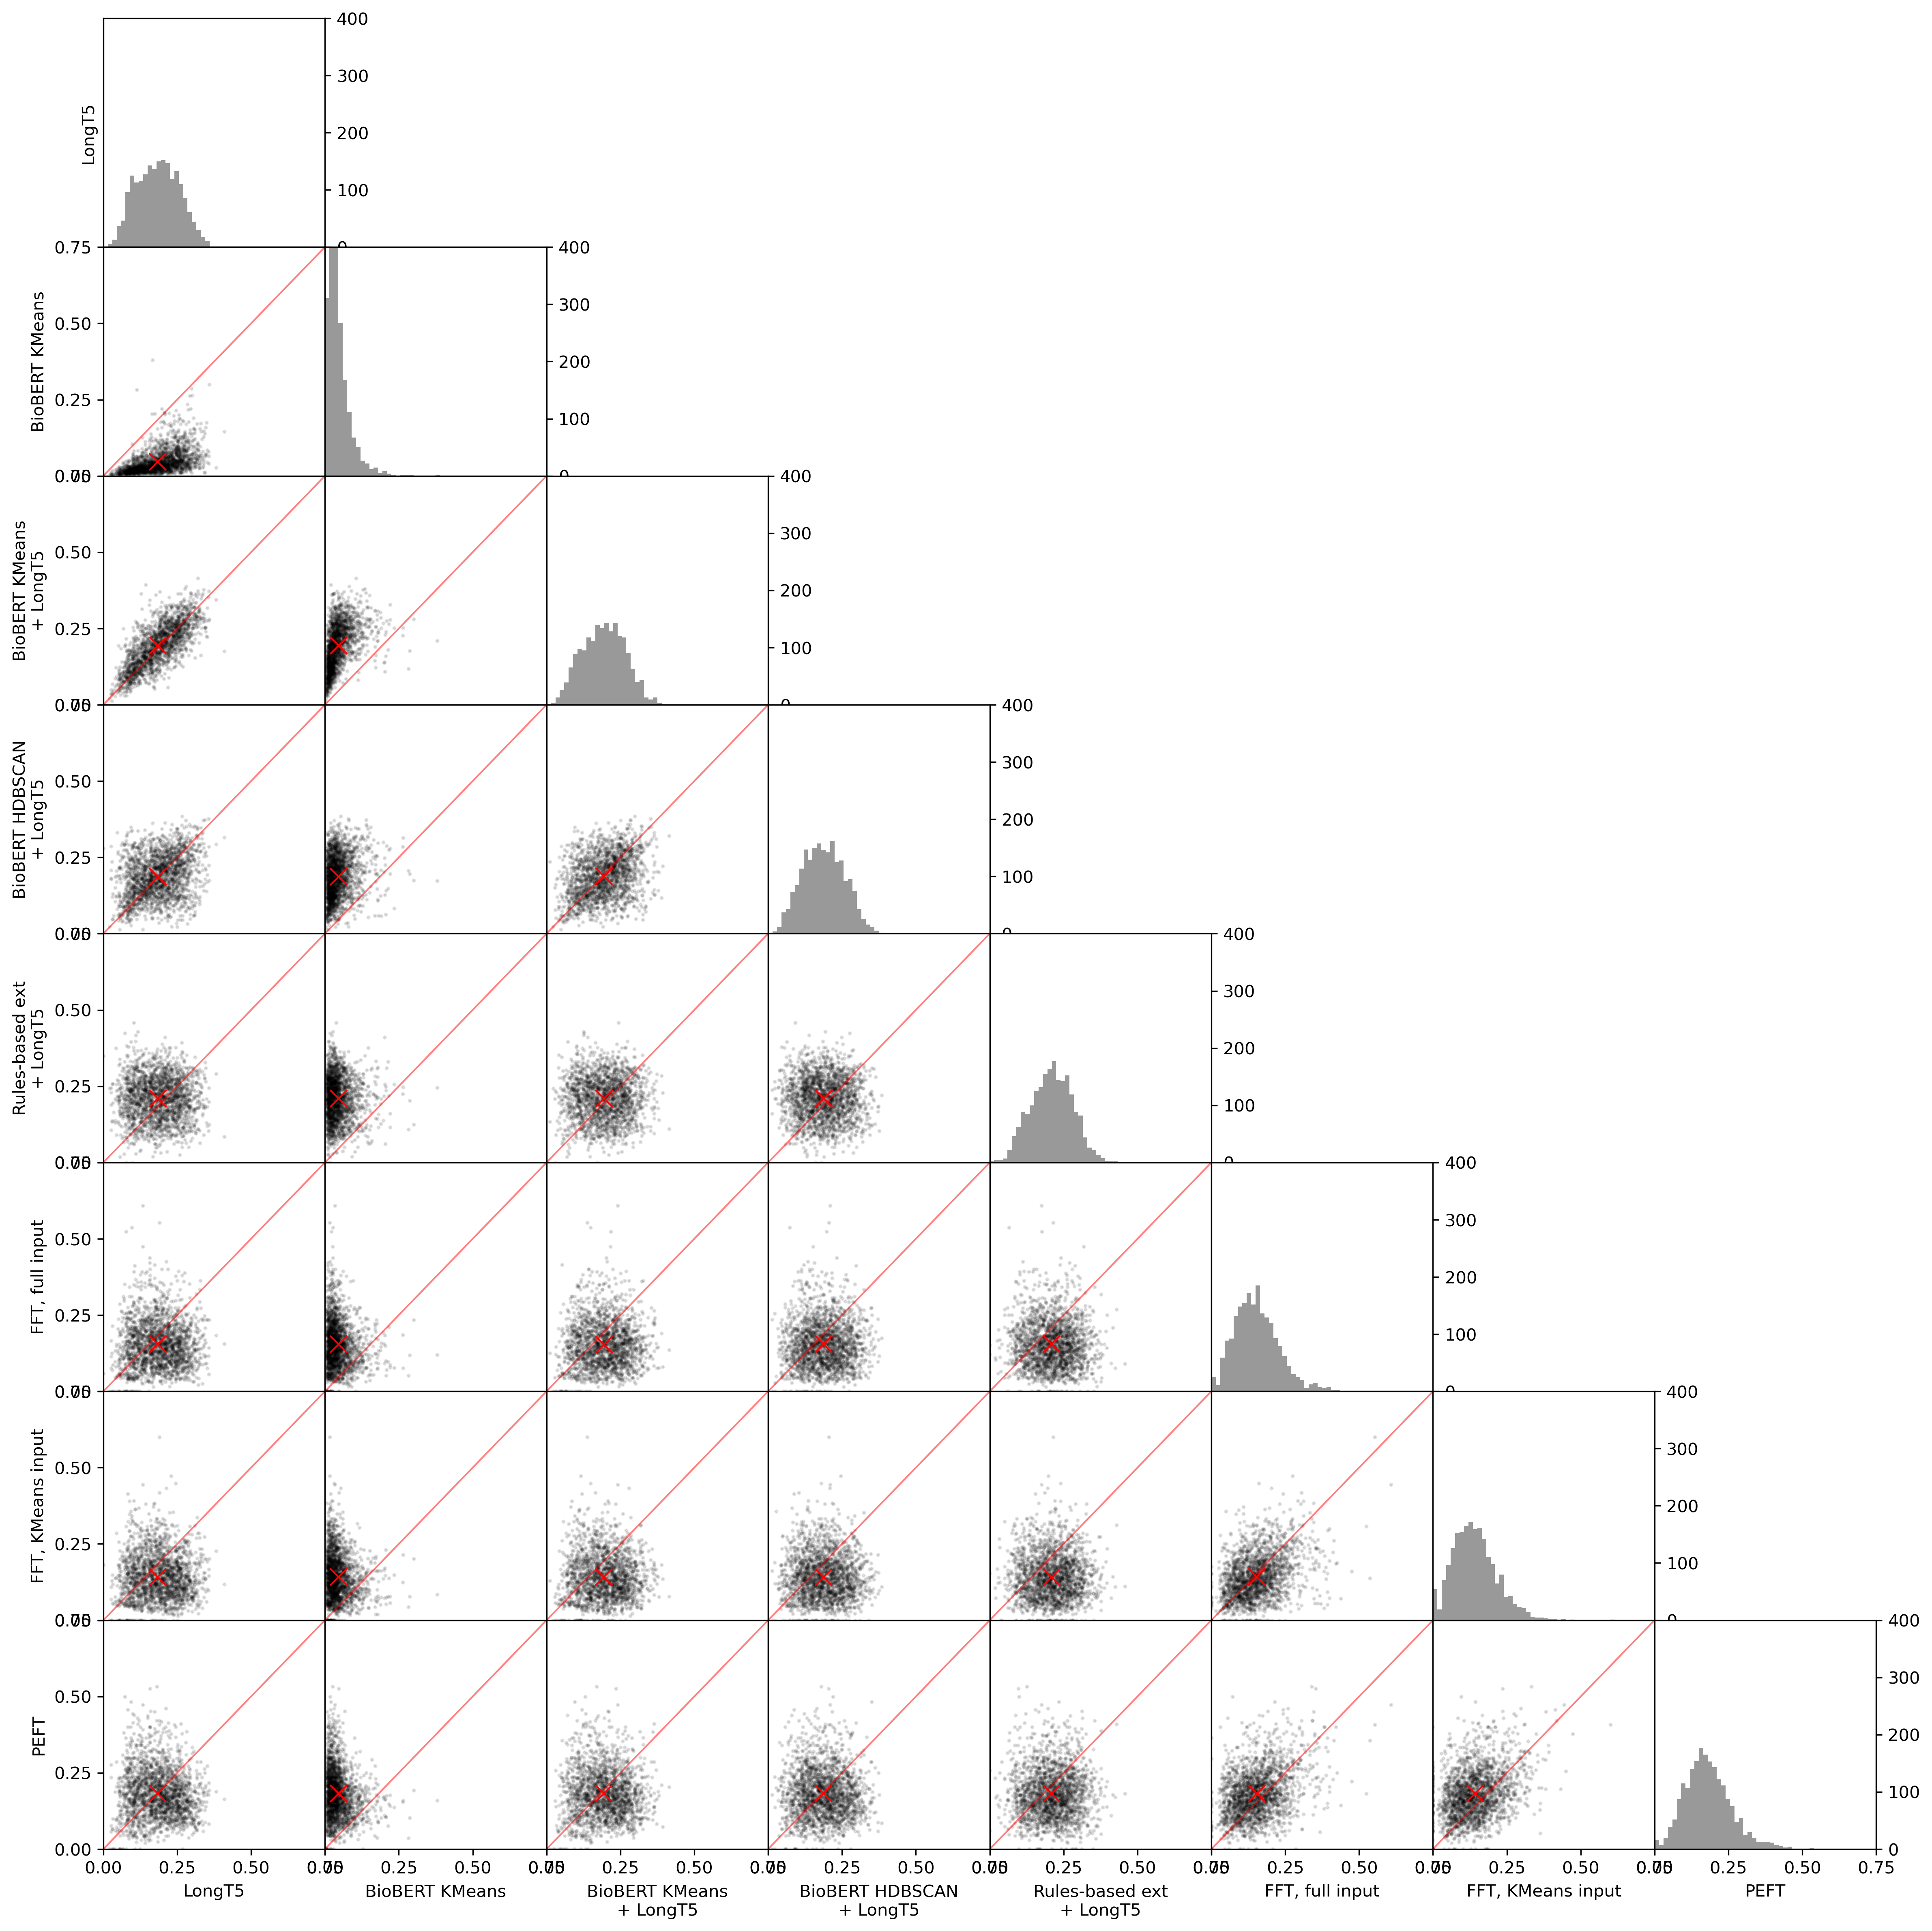
\includegraphics[width=\linewidth]{scatterplot_ROUGE-rouge1-fmeasure.png}
  \captionof{figure}{Example-level comparison of ROUGE-1 F1.}
  \label{fig:pair-rouge1}
\end{center}
\begin{center}
  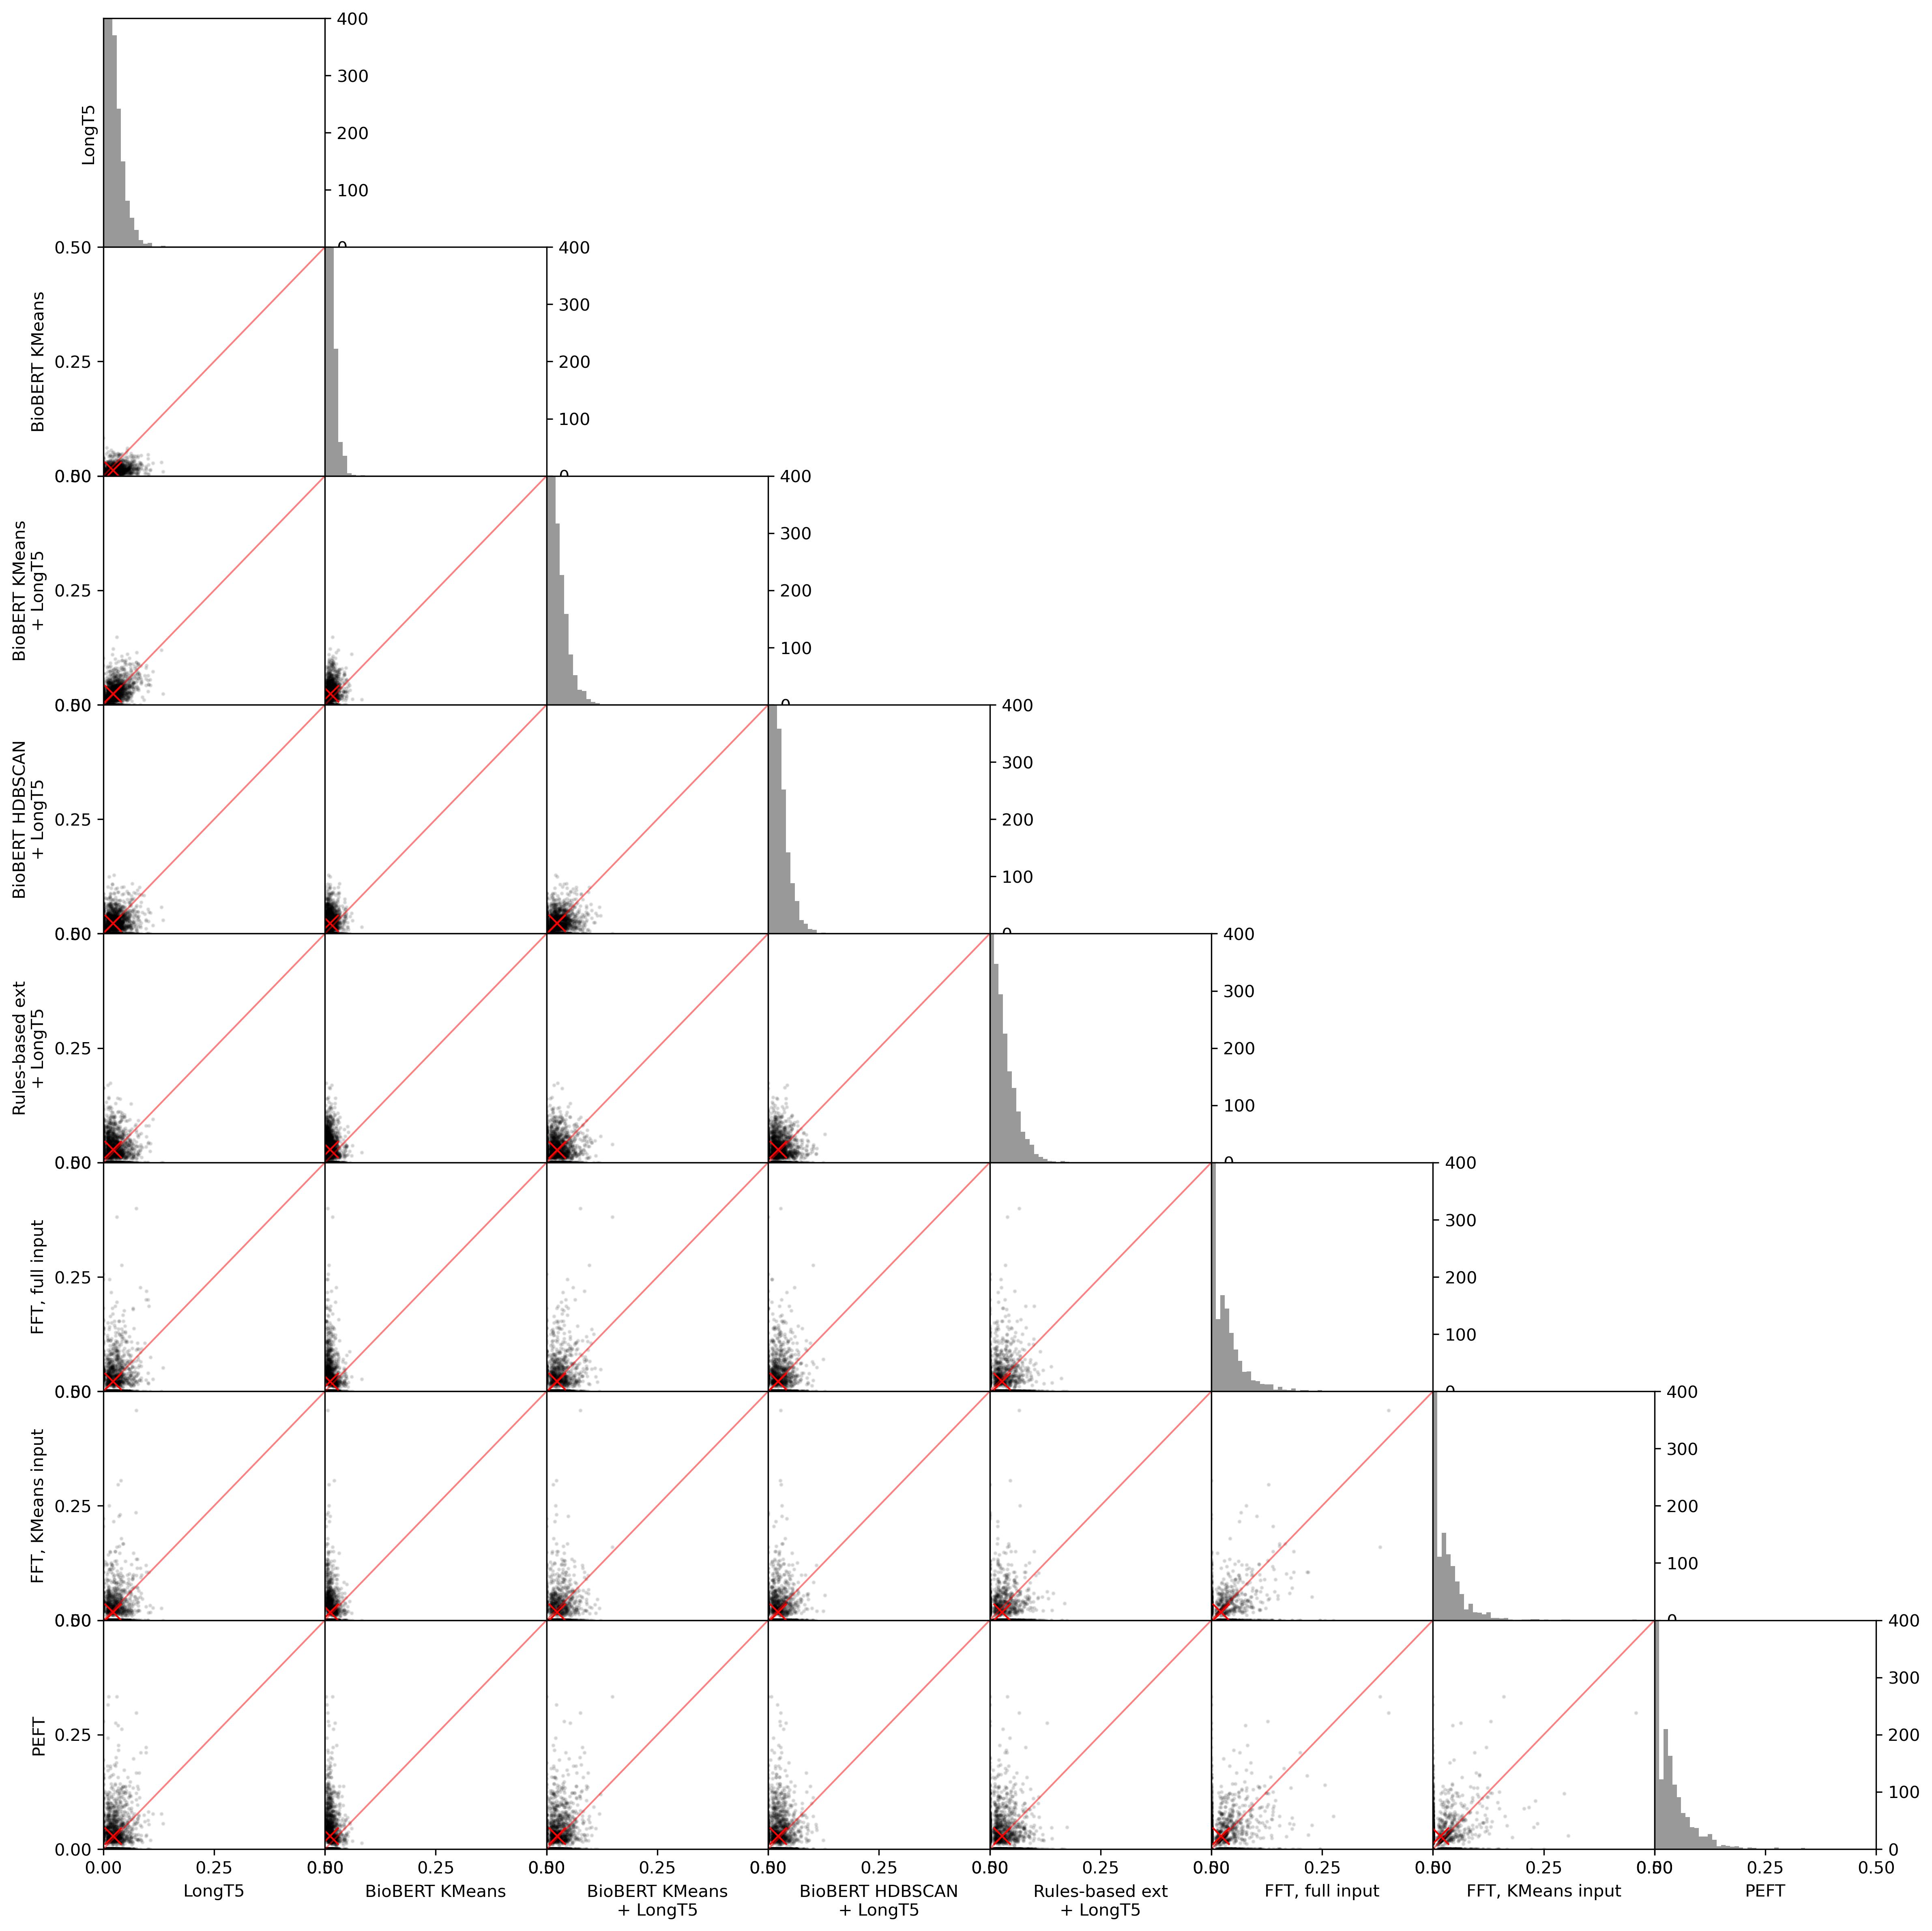
\includegraphics[width=\linewidth]{scatterplot_ROUGE-rouge2-fmeasure.png}
  \captionof{figure}{Example-level comparison of ROUGE-2 F1.}
  \label{fig:pair-rouge2}
\end{center}
\begin{center}
  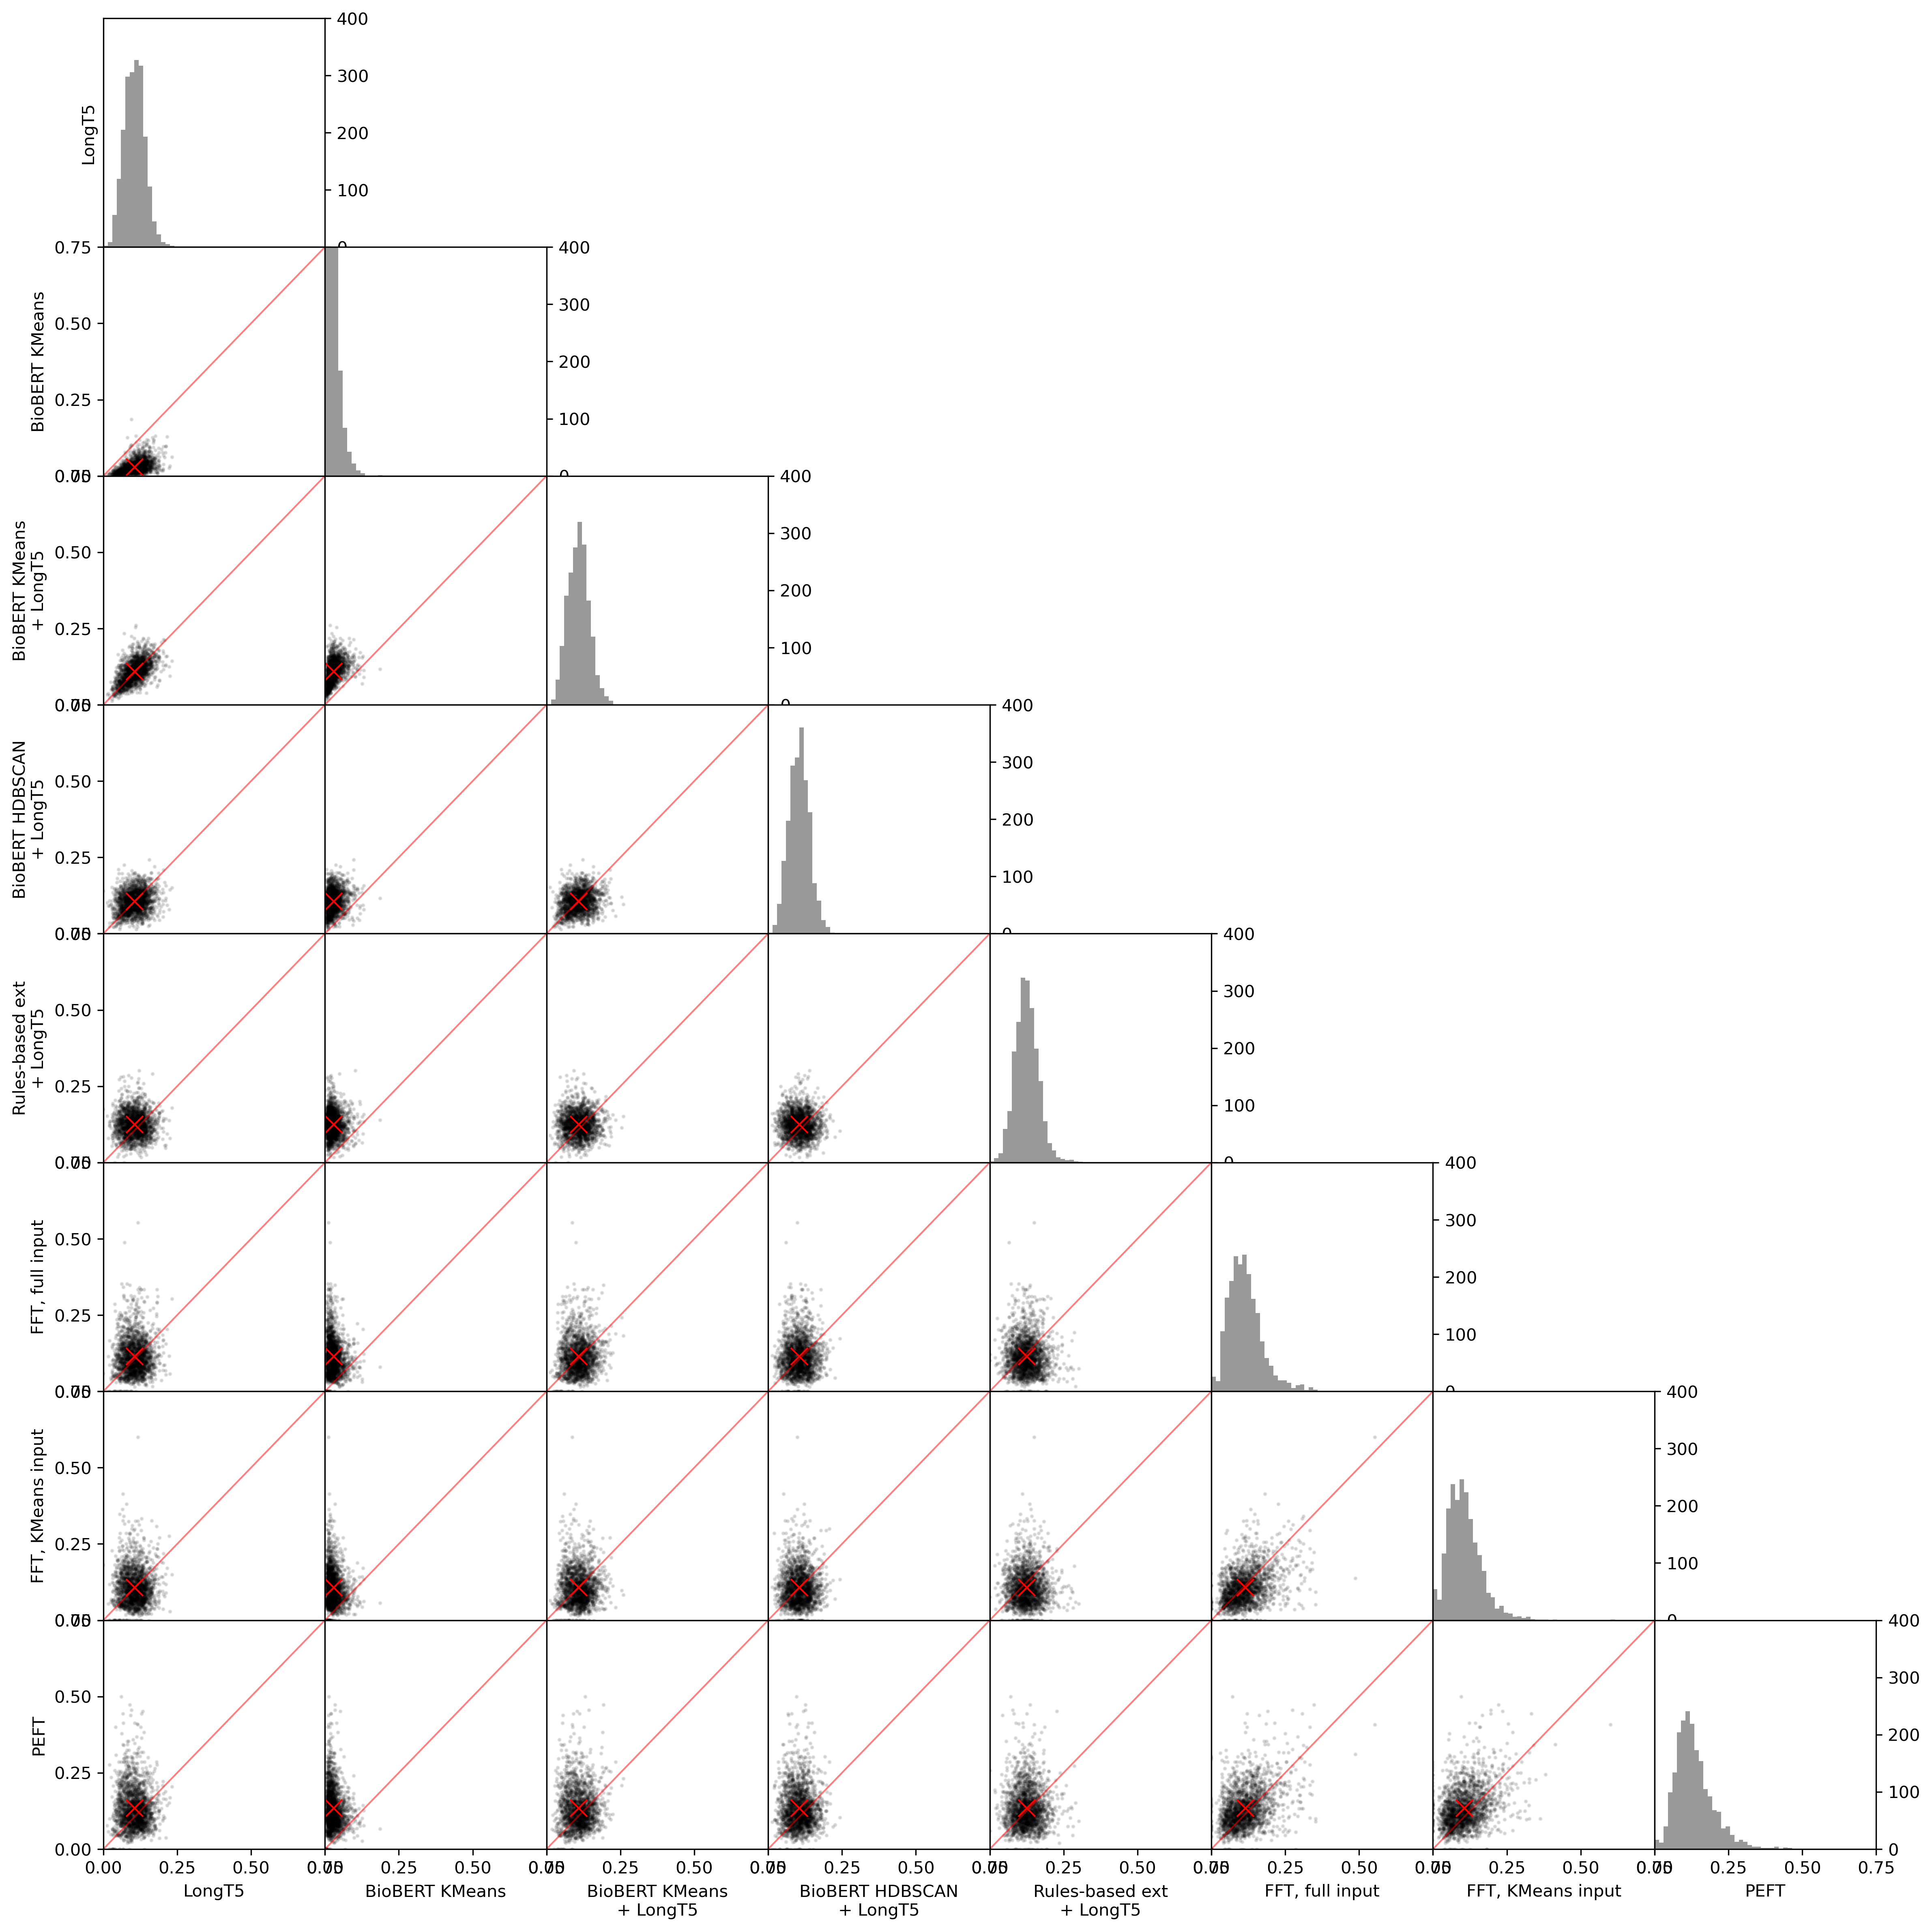
\includegraphics[width=\linewidth]{scatterplot_ROUGE-rougeL-fmeasure.png}
  \captionof{figure}{Example-level comparison of ROUGE-L F1.}
  \label{fig:pair-rougeL}
\end{center}
\begin{center}
  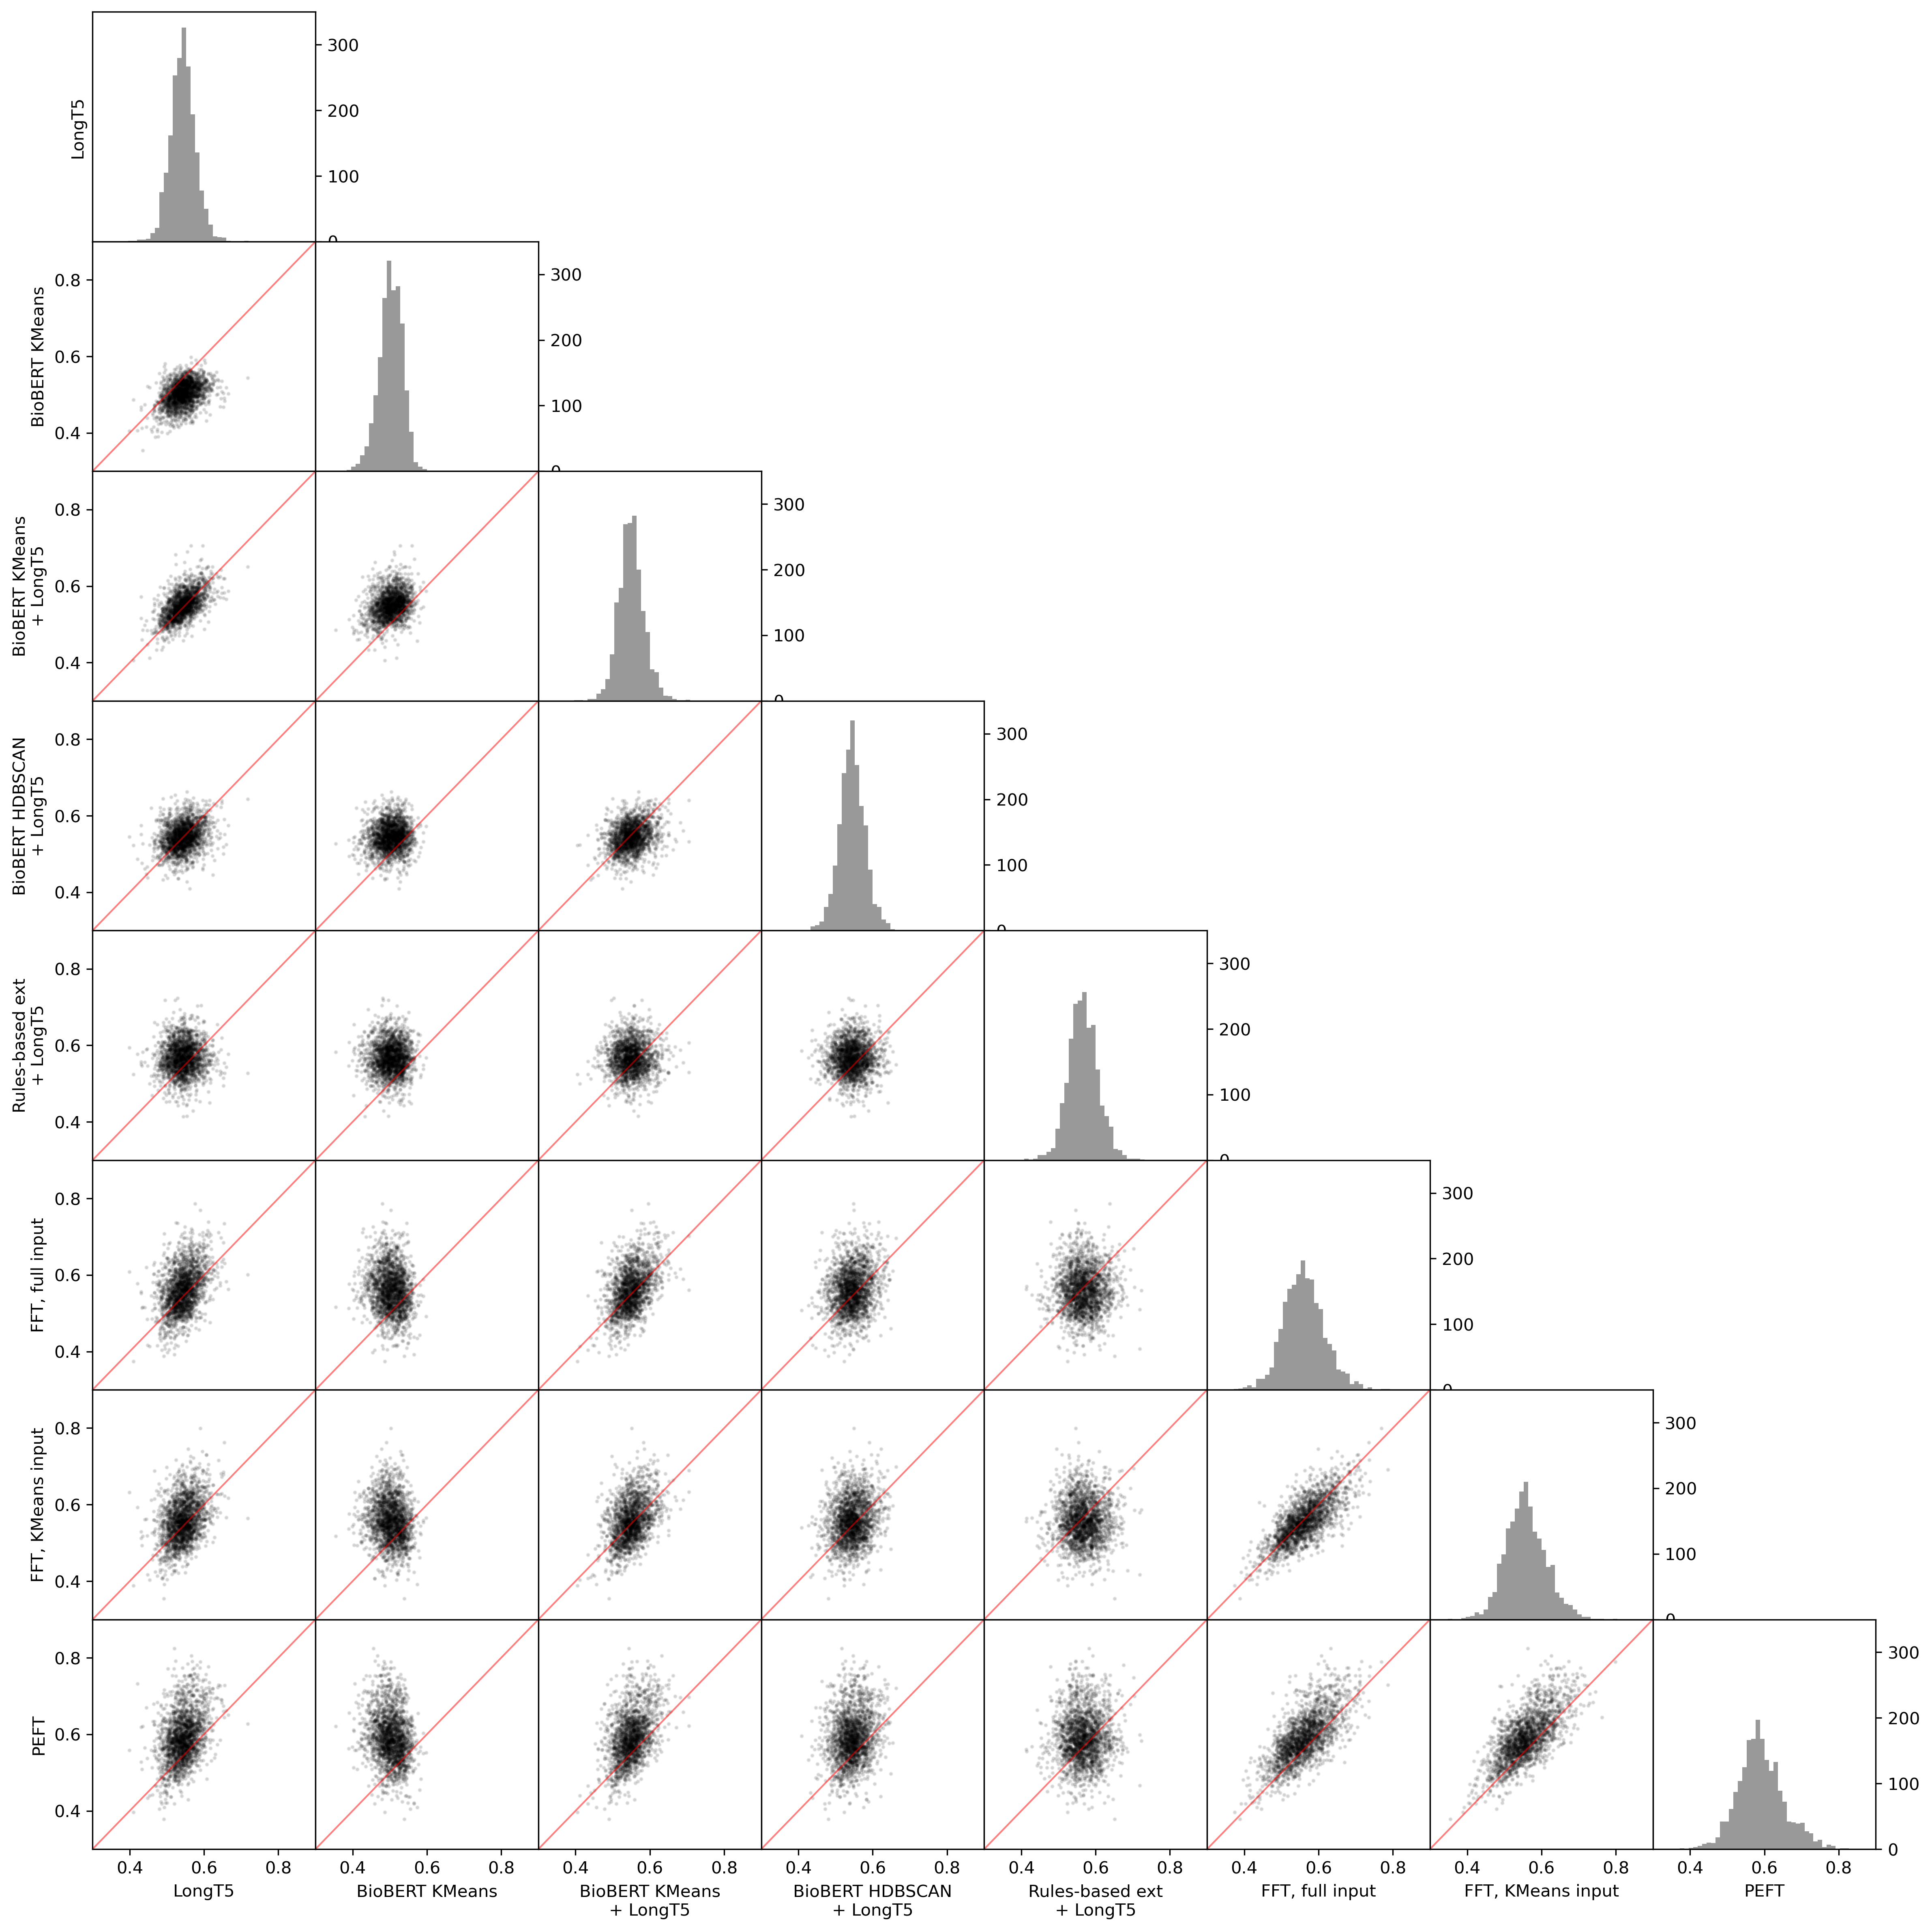
\includegraphics[width=\linewidth]{scatterplot_bertscore_f1s.png}
  \captionof{figure}{Example-level comparison of BERTscore F1.}
  \label{fig:pair-bertscore}
\end{center}
\begin{center}
  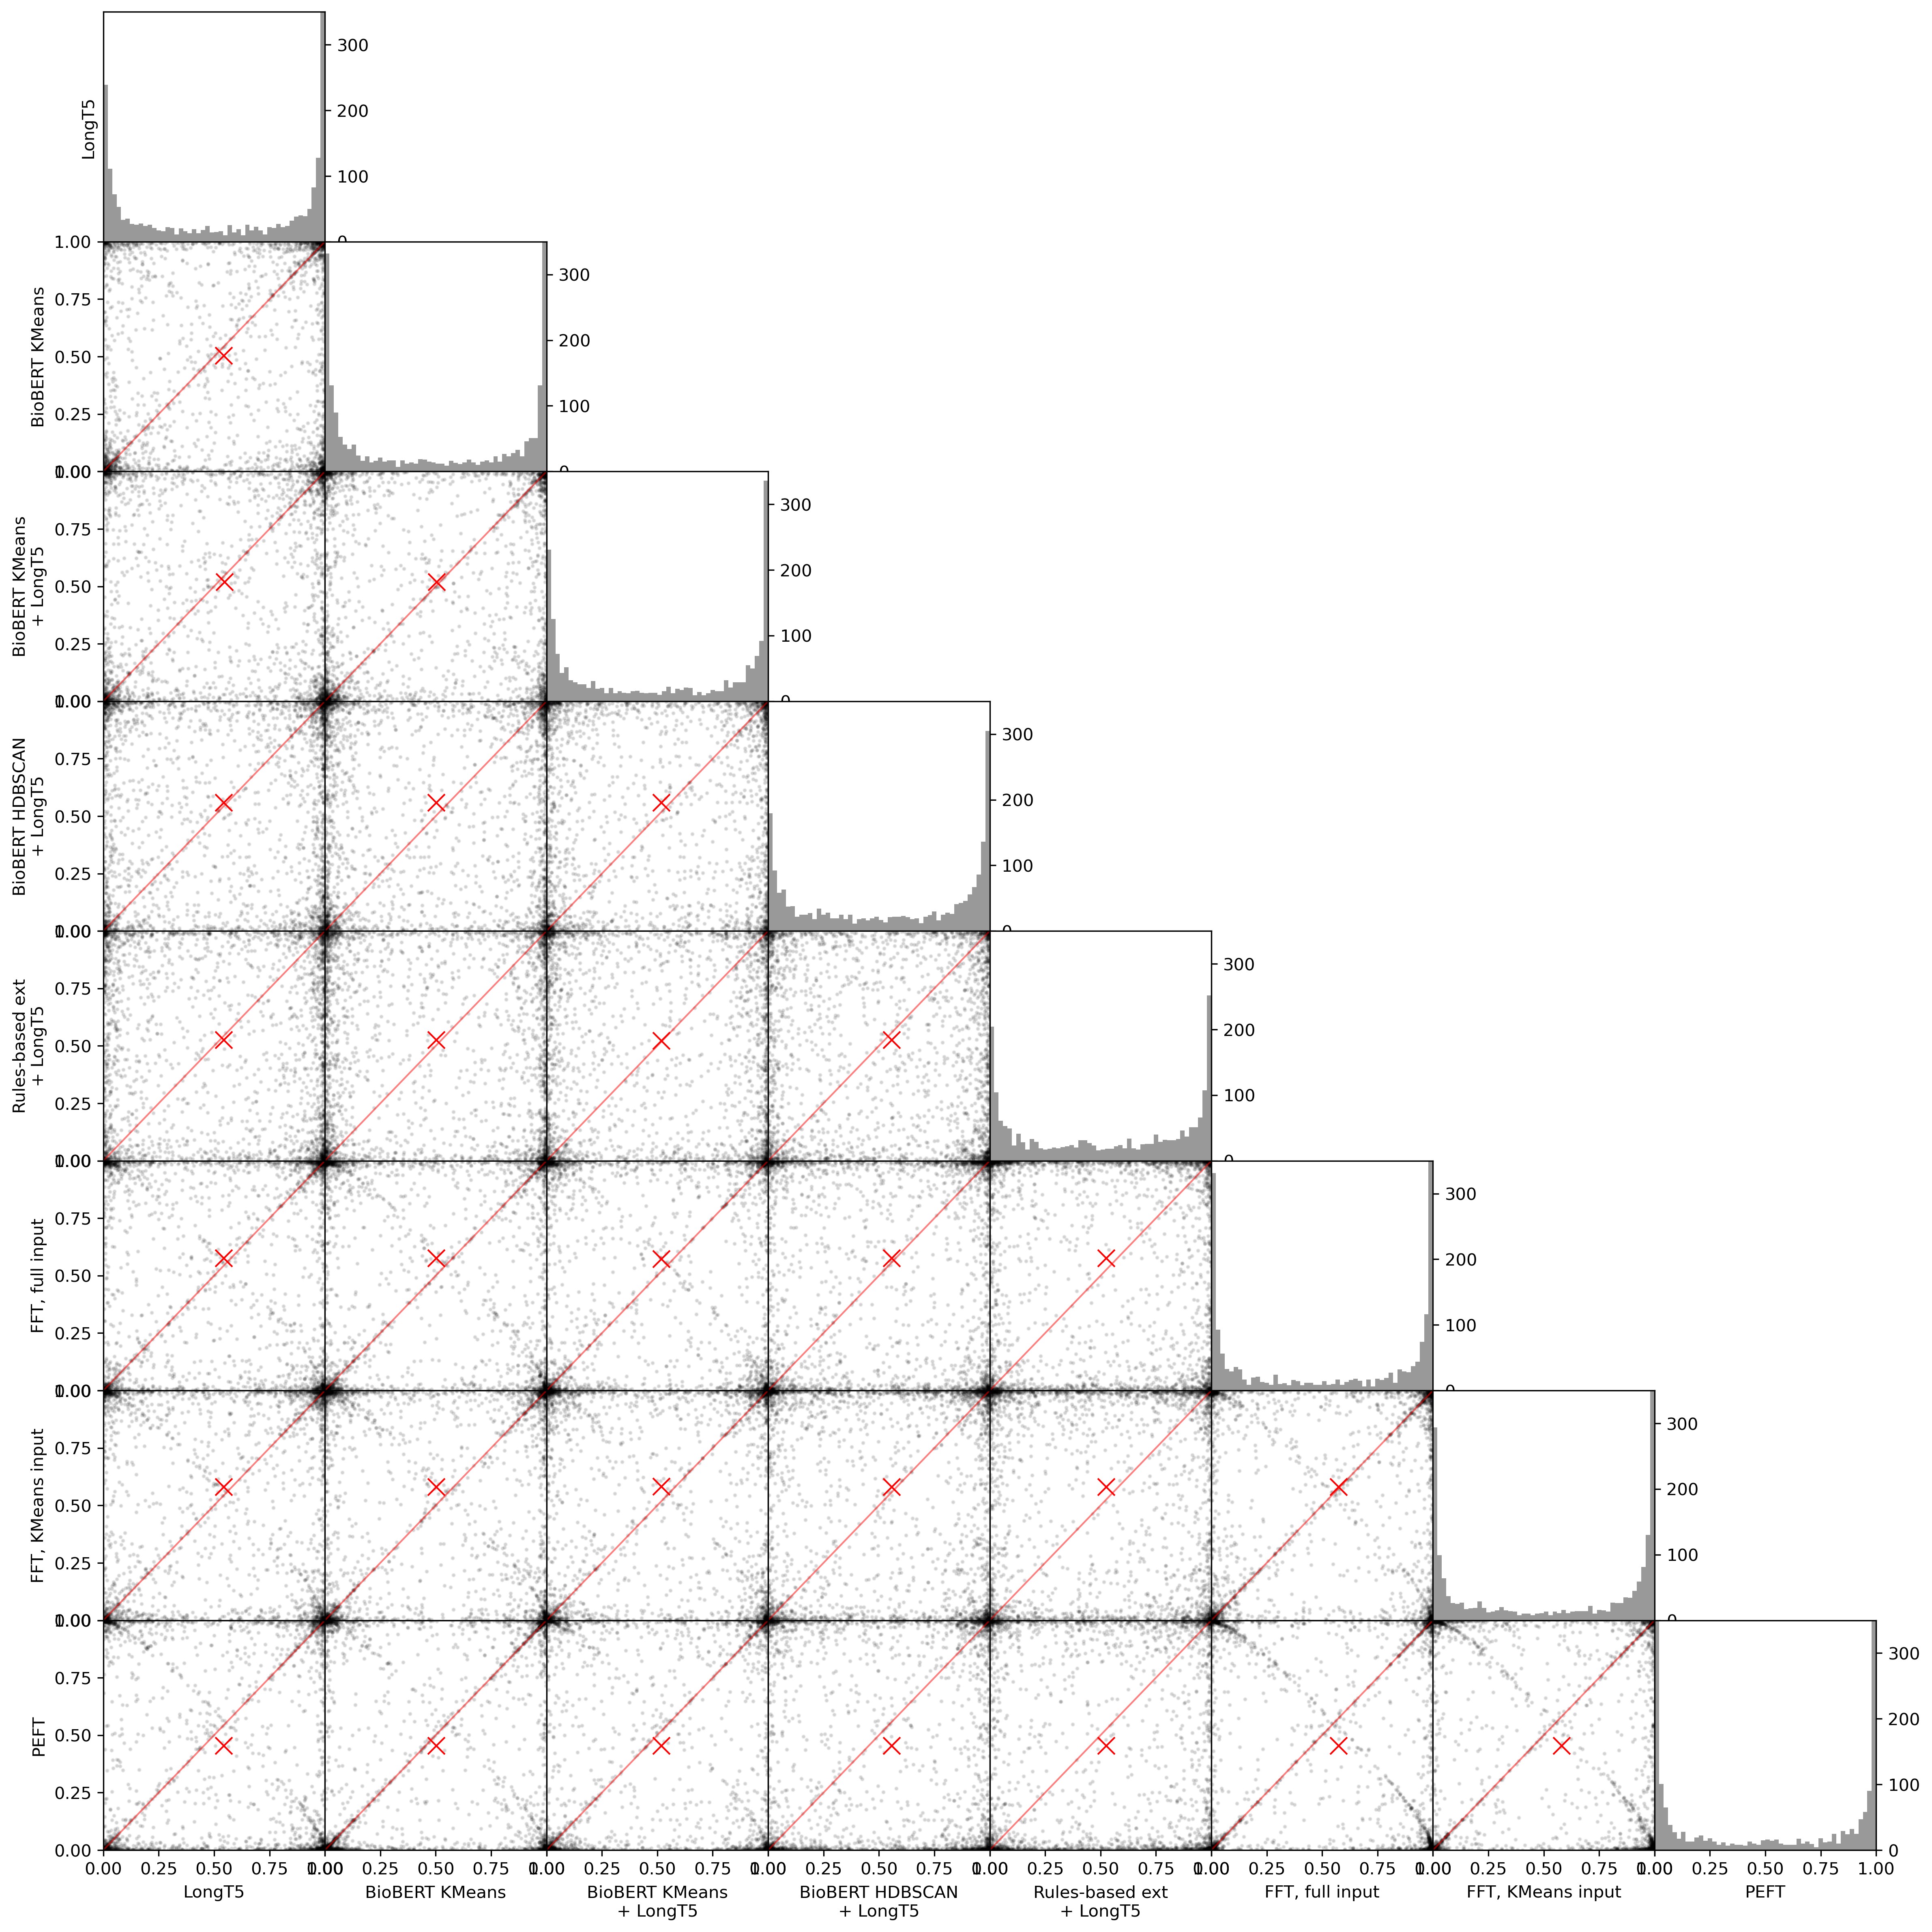
\includegraphics[width=\linewidth]{scatterplot_deltaEI.png}
  \captionof{figure}{Example-level comparison of $\Delta$EI.}
  \label{fig:pair-deltaEI}
\end{center}

\end{document}

